\begin{titlepage}
	\begin{center}
		\vspace*{1cm}
		
		
		
		
		\textbf{\Huge Analisi II}
		
		\vspace{0.8cm}
		Riassunto da: \textit{"Analisi Matematica 2 - Claudio Canuto, Anita Tabacco"}
		\vspace{0.5cm}
		
		\small{Dispensa realizzata da \textit{Federico Cesari} e \textit{Matteo Herz}}
	\vspace{4.5cm}
	
	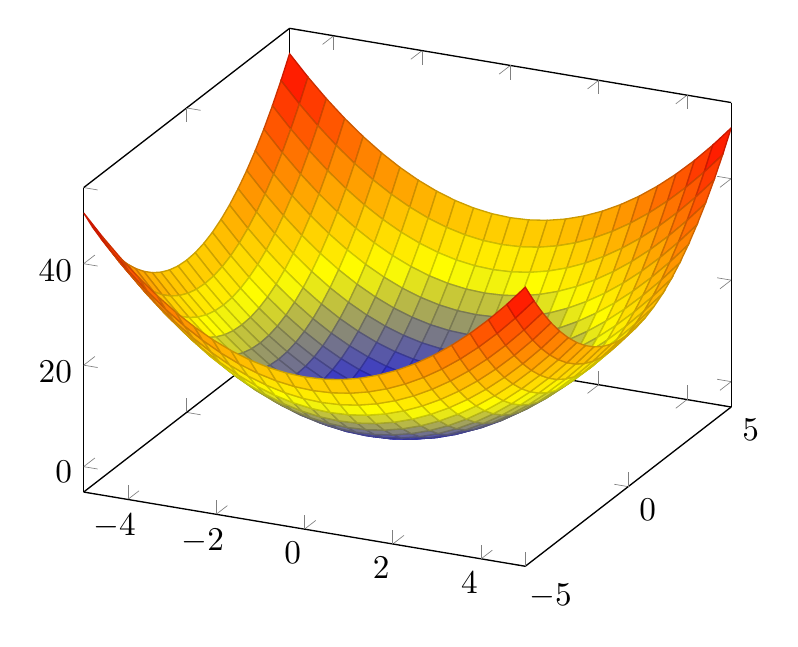
\begin{tikzpicture}[scale=1.2]
		
		\begin{axis}[ domain=-5:5, domain y=-5:5, title={} ]
			\addplot3[surf,samples=25] { x^2+y^2 };
		\end{axis}
		
	\end{tikzpicture}
	
	
	\vfill
	
	
	
	\vspace{0.8cm}
	
	
	Corso di Laurea in Fisica - Corso A\\
	Università degli studi di Torino, Torino\\
	Settembre 2024\\
	
	
\end{center}
\end{titlepage}
